\documentclass{article}

\usepackage{listings} % Required for inserting images
\usepackage{xcolor}
\usepackage{graphicx}

\lstset{
language = Python
 basicstyle=\ttfamily,
 keywordstyle=\color{purple},
 commentstyle=\color{green},
 stringstyle=\color{blue},
 showstringspaces=false,
 breaklines=true,
 tabsize=6,
 }
 
\begin{document}

Trabalho Matemática

Nome: Isabela Vieira Da Silva Cruz Martins

curso: Ciencia de dados


1) Deduza A o determinante 4x4 usando a formula
\begin{figure}[h]
    \centering
    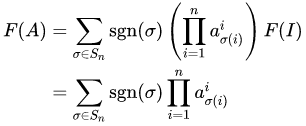
\includegraphics{Formula.png}
    \caption{Formula de Leibniz}
    \label{fig:exemplo}
\end{figure}

\begin{lstlisting}
    A = [a11 a12 a13 a14]
        [a21 a22 a23 a24]
        [a31 a32 a33 a34]
        [a41 a41 a43 a44]

det ( A ) =
            a11*a22*a33*a44 + a11*a23*a34*a42 + a11*a24*a32*a43
           + a12*a21*a34*a43 + a12*a23*a31*a44 + a12*a24*a33*a41
           + a13*a21*a32*a44 + a13*a22*a34*a41 + a13*a24*a31*a42
           + a14*a21*a33*a42 + a14*a22*a31*a43 + a14*a23*a32*a41
           - a11*a22*a34*a43 - a11*a23*a32*a44 - a11*a24*a33*a42
           - a12*a21*a33*a44 - a12*a23*a34*a41 - a12*a24*a31*a43
           - a13*a21*a34*a42 - a13*a22*a31*a44 - a13*a24*a32*a41
           - a14*a21*a32*a43 - a14*a22*a33*a41 - a14*a23*a31*a42
       
        
\end{lstlisting}
\begin{lstlisting}
 2) det(a) != 0 e det(a) = 0 
\end{lstlisting} 

\begin{lstlisting}
    a = [4 0 0 0]
        [1 0 1 1]
        [-6 6 1 3]
        [2 0 -1 1]

det(a) = -48

    a = [1 2 3 4]
        [2 4 0 8]
        [-1 -2 -3 -4]
        [2 5 8 11]

det(a) = 0        
        
\end{lstlisting}


3) O código que replica a formula de Leibinz em python:

\begin{lstlisting}
matriz = [[4, 0, 0, 0]],
         [1, 0, 1, 1],
         [-6, 6, 1, 3],
         [[2, 0, -1, 1]]

def leibniz(matriz) :
    n = len(matriz)
    if n == 1:
        return matriz[0][0]
    else:
        soma = 0
        for j in range(n):
            nova_matriz = []
            for i in range(1, n):
                linha = []
                for k in range(n):
                    if k != j:
                        linha.append(matriz[i][k])
                nova_matriz.append(linha)
            sinal = (-1) ** j
            soma += matriz[0][j] * sinal * leibniz(nova_matriz)
        return soma

determinante = leibniz(matriz)

print("O determinante da matriz :", determinante)
         \end{lstlisting}

Comprovando no console as duas matrizes do 2)

\begin{figure}
    \centering
    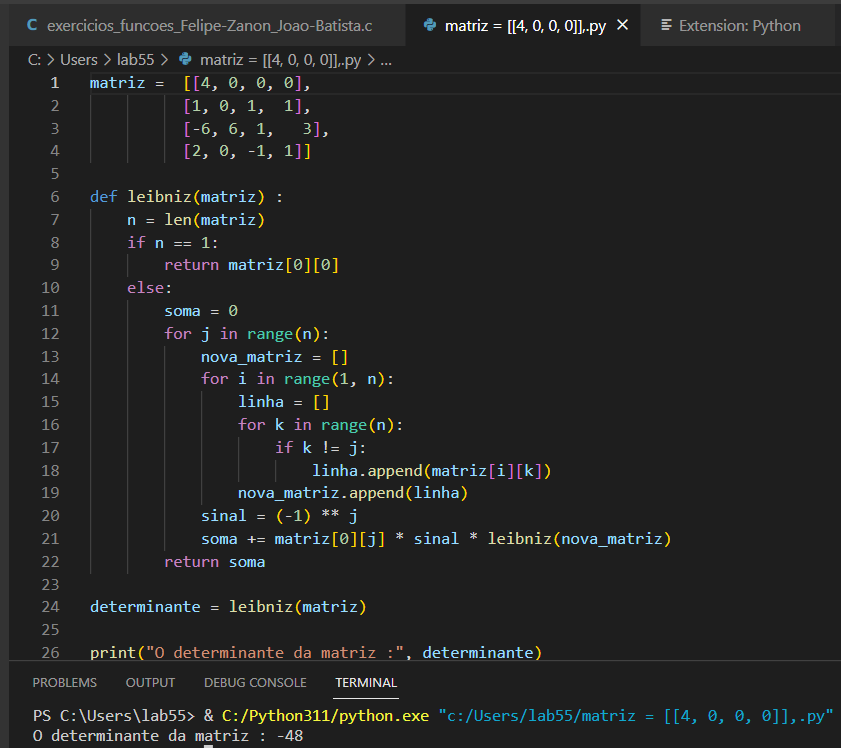
\includegraphics{Captura de tela 2023-05-09 105317.png}
    \caption{Caption}
    \label{fig:my_label}
\end{figure}
\end{document}

